\documentclass[12pt,a4paper]{article}

\usepackage{mathtools}
\usepackage{graphicx}
\usepackage{braket}
\usepackage{amsthm}
\usepackage{lmodern}
\usepackage[utf8]{inputenc}
\usepackage[frenchb]{babel}
\usepackage[T1]{fontenc}
\usepackage{subcaption}
\usepackage{caption}
\usepackage{gensymb}
\usepackage{tikz}
\usepackage{qcircuit}
\usepackage{listings}
\usepackage{pgfplots}
\usepackage{appendix}
\usepackage{hyperref}
\usepackage[ruled,vlined]{algorithm2e}
\usepackage{titlesec}
\usepackage{cleveref}
\usepackage{titling}
\usepackage{float}

\newtheorem{definition}{Définition}
\newtheorem{pb}{Problème}
\newtheorem{rem}{Remarque}
\newtheorem{ex}{Exemple}
\setlength{\droptitle}{-10em}

\title{Recuit Quantique}
\date{}

\begin{document}
\maketitle

\section{Opérateur Hamiltonien}
\subsection*{Modèle d'Ising}
Posons trois aimants $\{\sigma_1, \sigma_2, \sigma_3\}$ et notons $+1$ si ils indiquent \textit{Nord} et $-1$ si ils indiquent \textit{Sud}, par exemple:  "N - S - N" donne $\{+1, -1, +1\}$. L'énergie du système est alors la somme des interactions, donné par l'opérateur Hamiltonien. Dans le cas d'exemple, on aurait: $\mathcal{H} = \sigma_1 \sigma_2 + \sigma_2 \sigma_3$. On peut alors généraliser:  

$\mathcal{H} = \displaystyle\sum_{<i, j>} \sigma_i \sigma_j$, avec les $<i, j>$ paires d'aimants.

Maintenant, supposons qu'on puisse contrôler la force d'interaction entre les aimants. Cela introduit un nouveau terme $J_{ij}$ représentant cette force d'interaction. On peut alors écrire: 

$\mathcal{H} = \displaystyle\sum_{<i, j>} J_{ij} \sigma_i \sigma_j$.

Ensuite, on rajoute un champ magnétique global au système. Cela rajoute une interaction $h_i$ à chaque aimant $i$, on rajoute donc la somme des $h_i \sigma_i$ à l'expression. Par convention, on inverse les signes: 

$\mathcal{H} = -\displaystyle\sum_{<i, j>} J_{ij} \sigma_i \sigma_j - \displaystyle\sum_{i} h_i \sigma_i $.

On a donc les $J_{ij}$ représentant la force d'interaction entre les aimants, ou le \textit{couplage} du système, et les $h_i$ représentant le champ magnétique, ou le \textit{biais} du système.

On peut représenter l'énergie du système par un graphe, comme à la figure \ref{fig:energyGraph}: 

\begin{figure}[H]
    \centering
    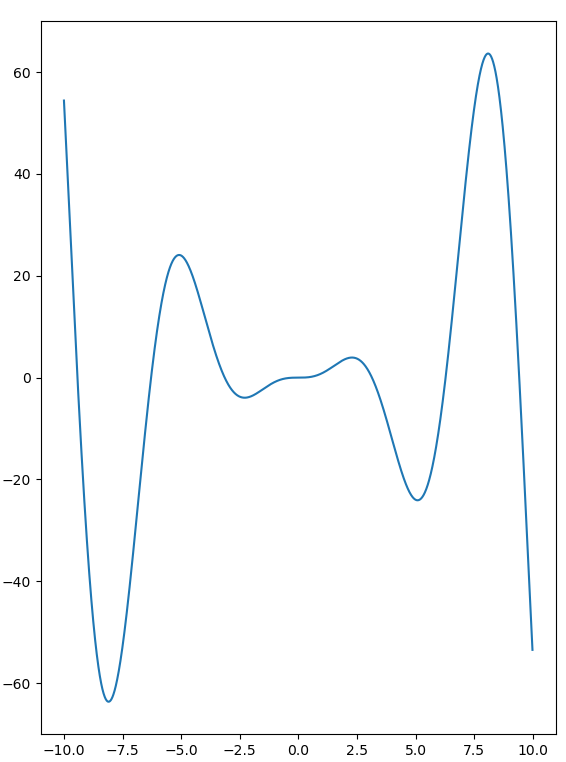
\includegraphics[scale=0.2]{ex_energy_graph.png}
    \caption{Exemple de graphe d'énergie}
    \label{fig:energyGraph}
\end{figure}


Naturellement, le système va tendre vers un état d'énergie minimum. En revanche, il peut se retrouver dans un minimum local, et ne pas avoir assez d'énergie pour sauter vers un état d'énergie plus bas.


\section{Recuit Quantique}
\subsection*{Principe général}
Le recuit quantique est l'analogue de la simulation de recuit en classique. A la place des gradients de température utilisés en classique pour passer d'un minimum local à un autre, on utilise en quantique la possibilité des systèmes quantiques de faire des sauts d'états, permettant potentiellement d'éviter de se retrouver bloqué dans un minimum local.

Dans le recuit quantique, on considère que la fonction de coût correspond à trouver l'état de base d'un Hamiltonien d'Ising $\mathcal{H}_0$ (vecteur d'état propre de $\mathcal{H}_0$ ayant la plus faible énergie). L'idée est de constituer un Hamiltonien évoluant au cours du temps:

\begin{equation}
    \mathcal{H}(t) = A(t) \mathcal{H}_0 + B(t) \mathcal{H}_1
\end{equation}

Au départ, on aura $B(t) = 0$ et $A(t) = 1$. En faisant évoluer le système, on obtient à la fin de l'évolution $B(t) = 1$ et $A(t) = 0$. Cela permet donc au système de passer progressivement du premier Hamiltonien $\mathcal{H}_1$ vers l'Hamiltonien d'Ising $\mathcal{H}_0$.

Tout d'abord, pour appliquer l'Hamiltonien d'Ising à un système quantique, on doit ré-écrire son équation pour transformer les termes individuels $\sigma_i$ en des matrices de Pauli Z $\sigma_i^z = \begin{bmatrix} 1 & 0 \\ 0 & -1 \\ \end{bmatrix}$:

\begin{equation}
    \mathcal{H}_0 = -\displaystyle\sum_{<i, j>} J_{ij} \sigma_i^z \sigma_j^z - \displaystyle\sum_{i} h_i \sigma_i^z
\end{equation}

Comme cet Hamiltonien final correspond au modèle d'Ising classique, uniquement composé de matrices de Pauli Z (donc commutable), son état de base encode le résultat du problème.

\medbreak

On écrit ensuite l'Hamiltonien utilisé au départ:

\begin{equation}
    \mathcal{H}_1 = - \displaystyle\sum_{i} g_i \sigma_i^x
\end{equation}

On introduit ici la matrice de Pauli X de façon à avoir un système non-commutable au cours de l'évolution quand $\mathcal{H}(t)$ est composé à la fois de $\mathcal{H}_0$ et de $\mathcal{H}_1$. On utilise cet Hamiltonien car son état de base correspond à l'état superposé équiprobable, qui nous est facile à créer.

\subsection*{Théorème adiabatique quantique}
L'évolution d'un système quantique au cours du temps nous est donné par l'équation de Schrödinger:

\begin{equation}
    i \frac{d}{dt} \ket{\psi(t)} = \mathcal{H}(t) \ket{\psi(t)}
\end{equation}

où $\ket{\psi(t)}$ est le vecteur d'état dépendant du temps, et $\mathcal{H}(t)$ est l'Hamiltonien dépendant du temps. Pour chaque temps $t$, l'Hamiltonien $\mathcal{H}(t)$ possède un vecteur d'état de base $\ket{\psi_g (t)}$ étant le vecteur d'état propre ayant la plus faible énergie.

Le théorème adiabatique stipule que si $\mathcal{H}(t)$ évolue suffisament lentement, alors le vecteur d'état évoluant $\ket{\psi(t)}$ va rester proche du vecteur de base $\ket{\psi_g (t)}$.

% \subsection*{Modèle quantique: champ transverse}

% On peut prendre l'opérateur $\sigma^z = \begin{bmatrix} 1 & 0 \\ 0 & -1 \\ \end{bmatrix}$. On peut l'appliquer aux qubits $\ket{0}$ et $\ket{1}$: $\sigma^z \ket{0} = \ket{0}$; $\sigma^z \ket{1} = -\ket{1}$. Cet opérateur permet donc de retranscrire la notation $+1/-1$ de l'exemple des aimants ci-dessus. En fait, ici l'Hamiltonien peut être réécrit $\mathcal{H} = -\displaystyle\sum_{<i, j>} J_{ij} \sigma_i^z \sigma_j^z - \displaystyle\sum_{i} h_i \sigma_i^z $, mais tout les termes sont commutatifs, on est dans un système purement classique.

% On peut alors introduire un nouvel opéateur, $\sigma^x = \begin{bmatrix} 0 & 1 \\ 1 & 0 \\ \end{bmatrix}$. On a alors les multiplications $\sigma^x \sigma^z = \begin{bmatrix} 0 & -1 \\ 1 & 0 \\ \end{bmatrix}$ et $\sigma^z \sigma^x = \begin{bmatrix} 0 & 1 \\ -1 & 0 \\ \end{bmatrix}$ non égaux.

% On ré-écrit donc l'opérateur Hamiltonien de la façon suivante pour prendre en compte l'opérateur $\sigma^x$:

% $\mathcal{H} = -\displaystyle\sum_{<i, j>} J_{ij} \sigma_i^z \sigma_j^z - \displaystyle\sum_{i} h_i \sigma_i^z - \displaystyle\sum_{i} g_i \sigma_i^x$. 

% La dernière somme essaye de "pousser" le système à se placer dans un état de superposition, alors que les deux premiers cherchent à "pousser" le système dans un état déterminé correspondant à l'état d'énergie minimale.

\end{document}
